\section{Algorithm}

\subsection{Constraint Condition}
\begin{frame}
    \frametitle{Constraint Condition}
    \begin{itemize}
		\item Assume $n = 2^t$ for some integer $t \ge 0$ for all problems.
		\item The size of DP table is $n \times n$.
	\end{itemize}
\end{frame}

\subsection{Parenthesization Problem}
\begin{frame}
    \frametitle{Parenthesization Problem}
    \begin{figure}
		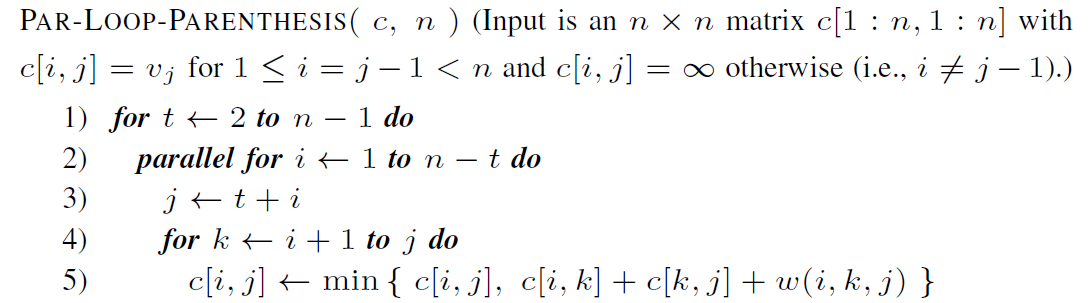
\includegraphics[scale=0.4]{figure/fig-parenthesis.png}
	\end{figure}
    \begin{itemize}
    	\item $w(i, k, j)$ returns the cost of combining parenthesizations of
    		$x_i \; \cdots x_k$ and $x_k \; \cdots x_j$
    	\item The optimal parenthesizing cost $c[1, n]$ for the entire sequence.
    \end{itemize}
\end{frame}

\subsection{Parenthesization Problem - Parallel CORDAC}
\begin{frame}
    \frametitle{Parallel CORDAC Algorithm - Func A, B}
    \begin{figure}
		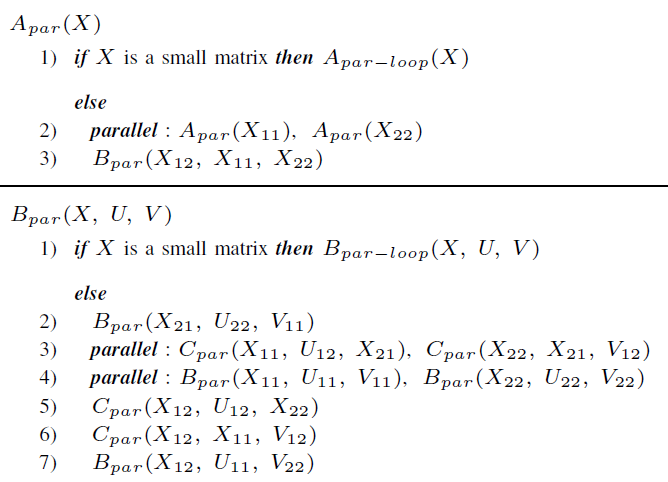
\includegraphics[scale=0.5]{figure/fig-parenthesis-parallel-1.png}
	\end{figure}
\end{frame}

\begin{frame}
    \frametitle{Parallel CORDAC Algorithm - Func C}
    \begin{figure}
		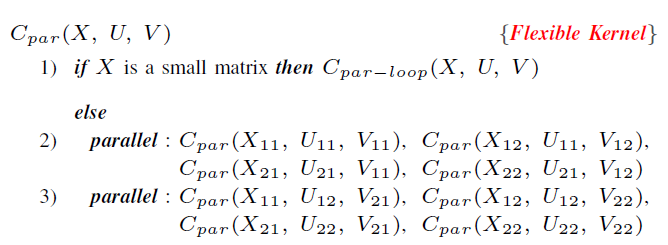
\includegraphics[scale=0.5]{figure/fig-parenthesis-parallel-2.png}
	\end{figure}
\end{frame}

\begin{frame}
    \frametitle{Parallel CORDAC Algorithm Figure}
    \begin{figure}
        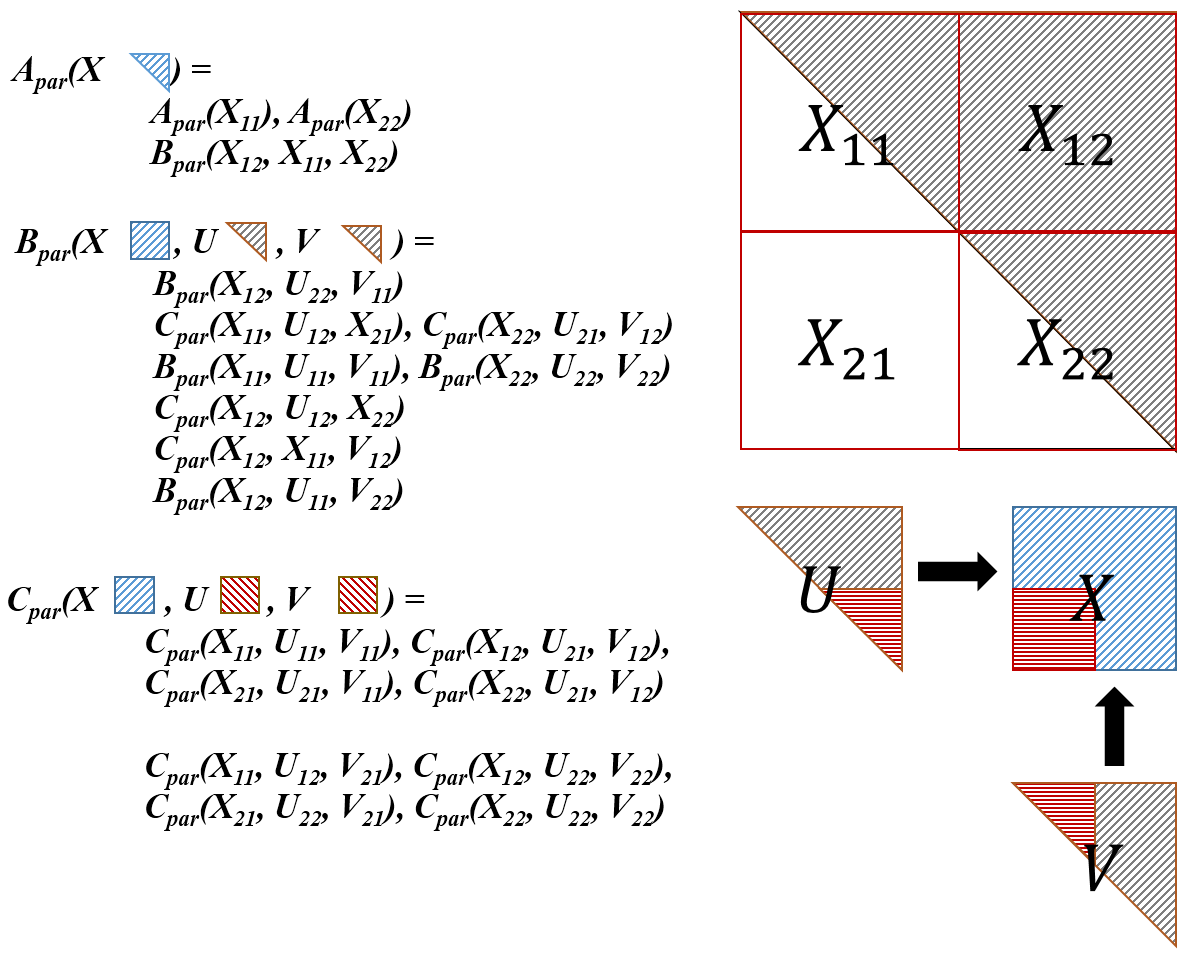
\includegraphics[scale=0.25]{figure/fig-par-explain.png}
    \end{figure}
\end{frame}

\subsection{Other Problems}
\begin{frame}
    \frametitle{Other Problems}
    \begin{figure}
		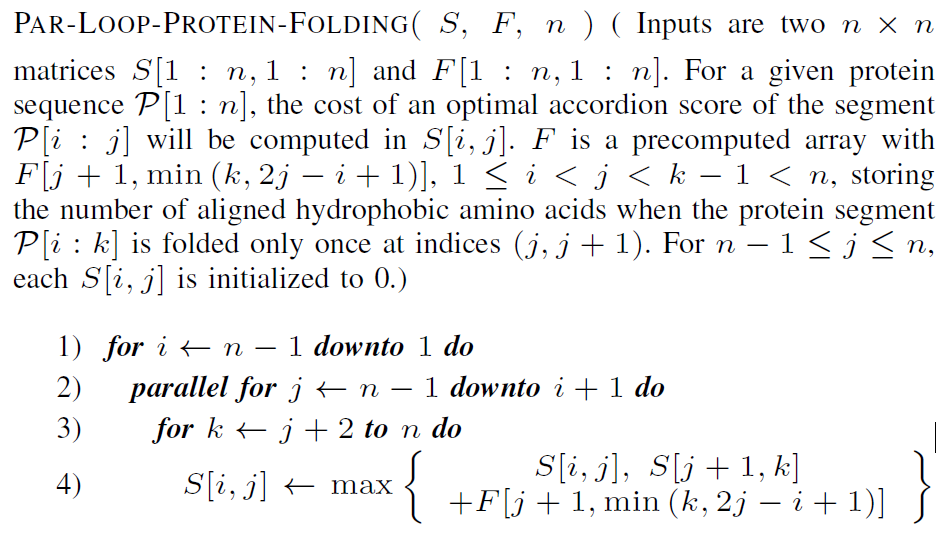
\includegraphics[scale=0.2]{figure/fig-folding.png}
	\end{figure}
	\begin{figure}
		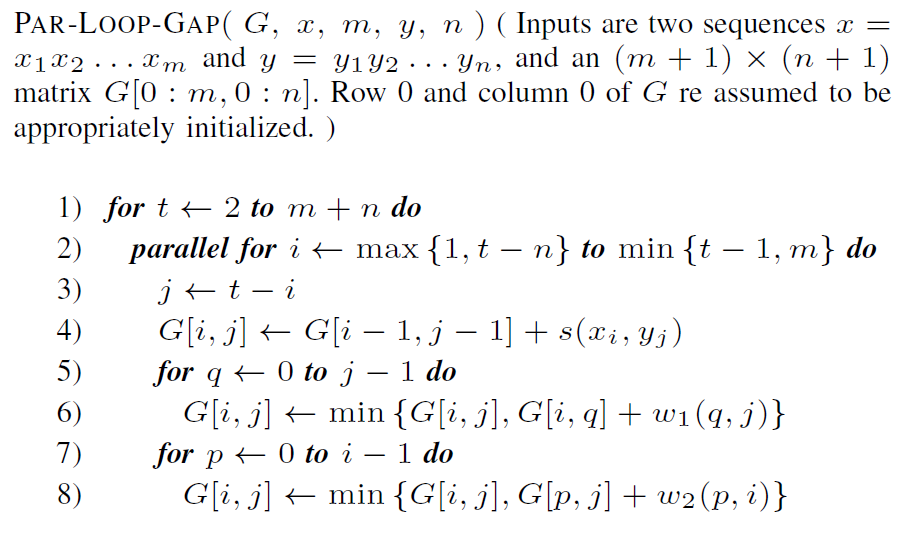
\includegraphics[scale=0.2]{figure/fig-gap.png}
	\end{figure}
\end{frame}

\subsection{Other Problems - Parallel CORDAC}
\begin{frame}
    \frametitle{Other Problems - Parallel CORDAC}
    \begin{figure}
		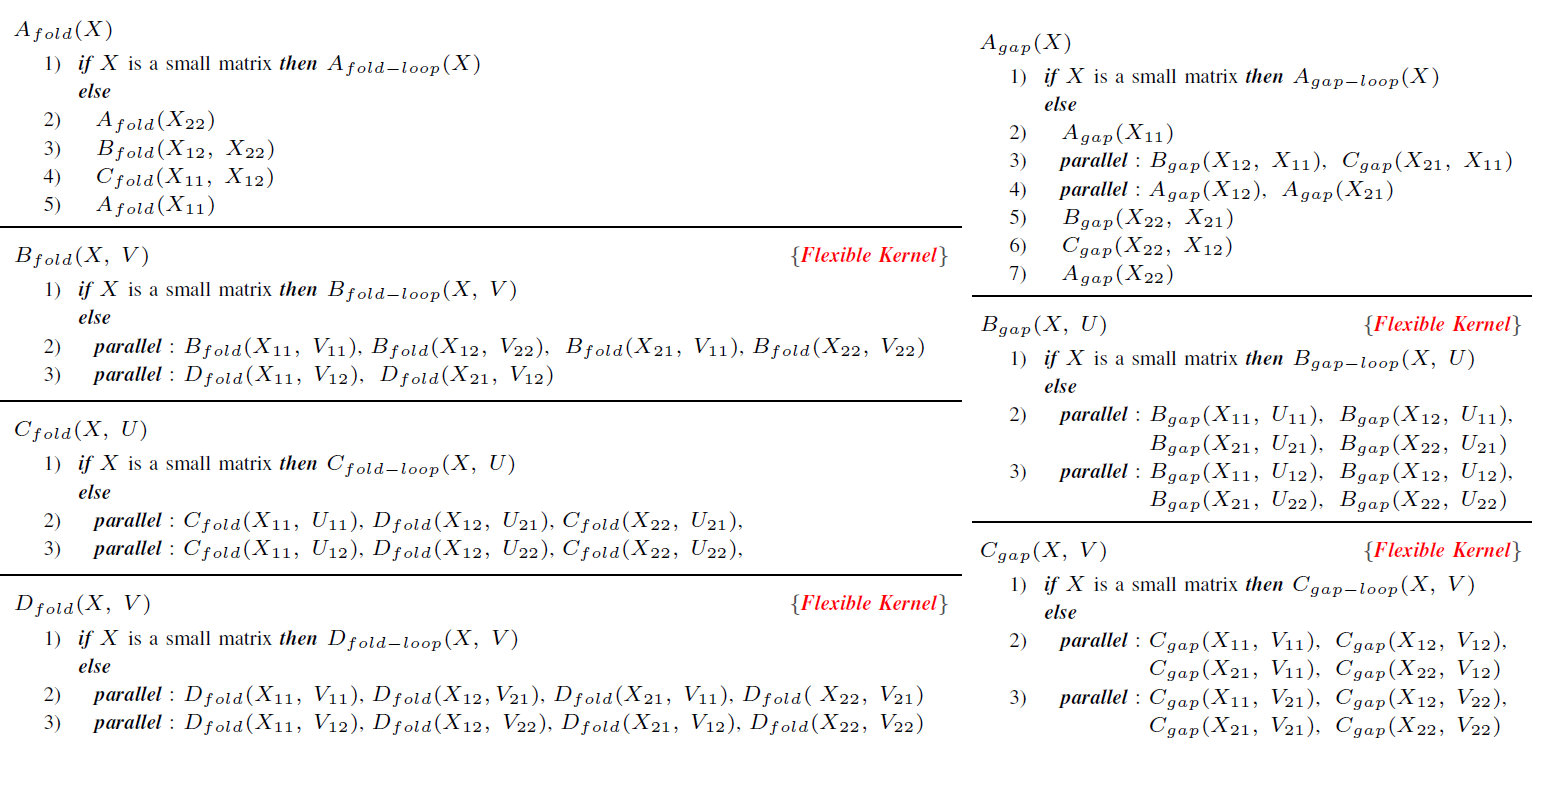
\includegraphics[scale=0.2]{figure/fig-fold-gap-parallel.png}
	\end{figure}
\end{frame}

\begin{frame}
    \frametitle{Other Problems - Parallel CORDAC}
    \begin{figure}
		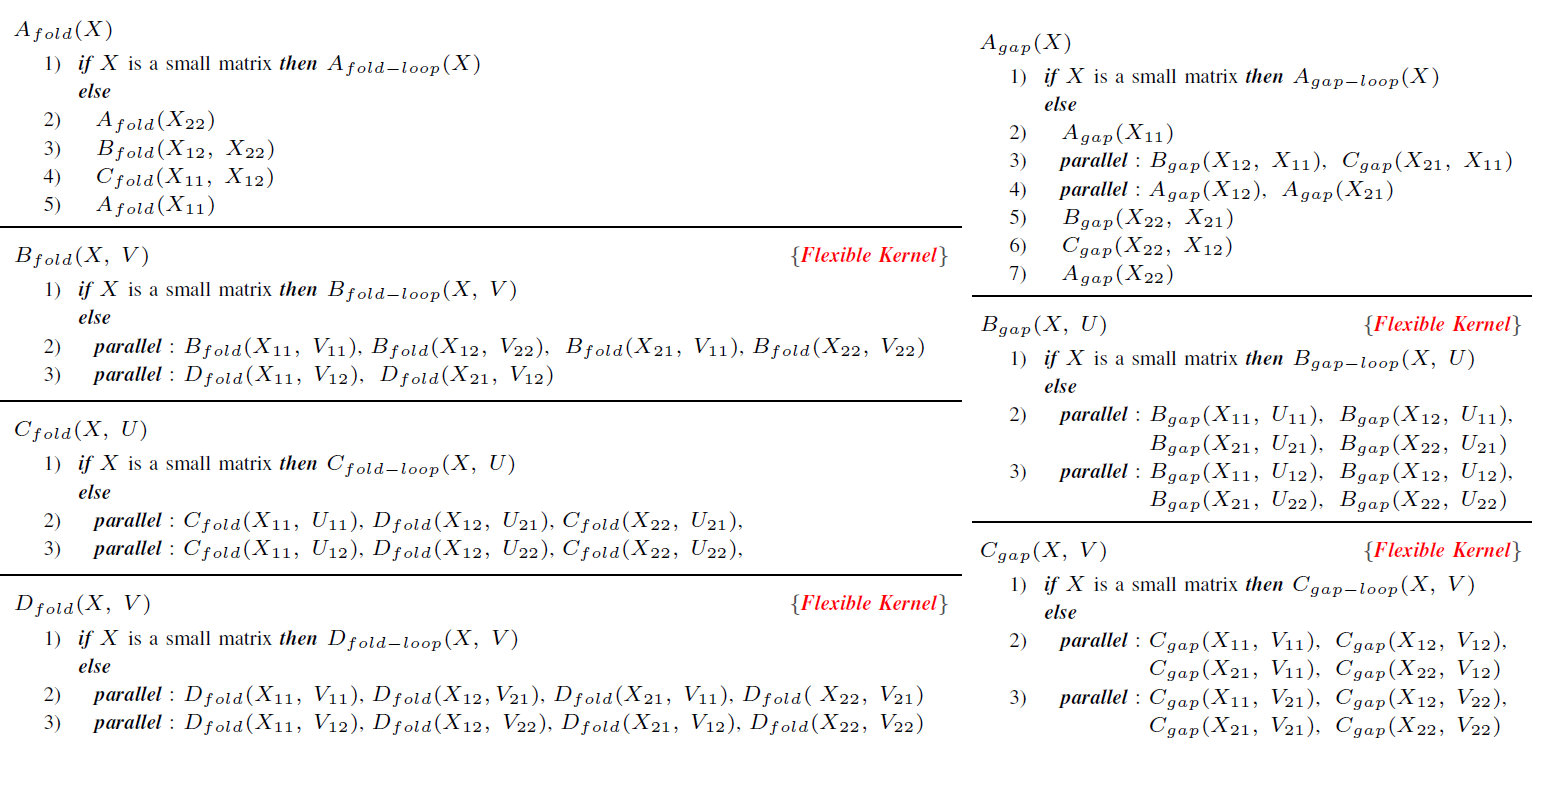
\includegraphics[scale=0.2]{figure/fig-fold-gap-parallel.png}
	\end{figure}
\end{frame}
